
\section{Лекция №3. Пределы измерений и <<Back Action>>}



% Раccмотрим спиновые измерения
% \begin{align*}
% 	\hat{\Pi}(0) &= \Pi_{00} \kb{0}{0} + \Pi_{01} \kb{1}{1}, \\
% 	\hat{\Pi}(1) &= \Pi_{10} \kb{0}{0} + \Pi_{11} \kb{1}{1}.
% \end{align*}

\subsection*{Пример линейного измерения}


Кстати, SQL -- Standart Quantum Limit, который даже достигнут и не является фундаментальным. Рассмотрим зеркало с координатой $x$, посылаем лучик, меряем фазу $\varphi$:
\begin{equation*}
	\sub{\varphi}{out} = \varphi + 2 k x
\end{equation*}
\textbf{Картина Гейзенберга}. Лучик описывается $\hat{N},\, \hat{\varphi}$, хотя оператора фазы и не бывает, но можно ввести оператор $\cos \hat{\varphi}$ и $\sin \hat{\varphi}$, с ненулевым коммутатором $\sim  \kb{0}{0} $. Поэтому для достаточно возбужденных состояний можно приближенно ввести оператор фазы канонически сопряженный числу квантов $N$
\begin{equation*}
	\left[\hat{N},\, \hat{\varphi}\right] = i.
\end{equation*}
Вполне естественно рассматривать гамильтониан
\begin{equation*}
	\hat{H} = - \hat{F} \hat{x} = - 2 \frac{\hbar \omega \hat{\dot{N}}}{c} \hat{x} = - 2 \hbar k \hat{\dot{N}} \hat{x}.
\end{equation*}
Посчитав уравнение Гейзенберга для этого гамильтониана
\begin{align*}
	\sub{\hat{\varphi}}{out} &= \hat{\varphi} + 2 k \hat{x} \\
	\sub{\hat{p}}{out} &= \hat{p} + 2 \hbar k \hat{N}
\end{align*}
Таким образом можем оценить координату $x$
\begin{equation*}
	\tilde{x} = \frac{\sub{\hat{\varphi}}{out}}{2k} = \hat{x} + \frac{\hat{\varphi}}{2k}.
\end{equation*}
Есть два линейных уравнения, все масштабы нелинейности (здесь $\lambda$) много больше величин, которые хотим померять, и это приводит к очень приятным последствиям. Действительно, рассмотрим
\begin{equation*}
	\left[\tilde{x},\, \sub{\hat{p}}{out} \right] = \left[\hat{x},\, \hat{p}\right] + \hbar \left[\hat{\varphi},\, 2k \hat{N}\right] = i \hbar + \hbar (-i) = 0,
\end{equation*}
что очень характерно для линейных систем.

Ошибка измерения
\begin{equation*}
	\langle \sub{(\Delta x)^2}{meas} \rangle = \frac{(\Delta \varphi)^2}{4 k^2} \overset{\mathrm{coh}}{=} \frac{1}{16 k^2 N},
\end{equation*}
где для когерентного состояния $\Delta N = N^{1/2}$ и $\Delta \varphi = \frac{1}{2} N^{-1/2}$.

И для обратного действия
\begin{equation*}
	\langle \sub{(\Delta p)^2}{BA} \rangle = 4 \hbar^2 k^2 (\Delta N)^2 \overset{\mathrm{coh}}{=}  4 \hbar^2 k^2 N. 
\end{equation*}
К слову, соотношение неопределенности
\begin{equation*}
	\langle \sub{(\Delta x)^2}{meas} \rangle 
	\langle \sub{(\Delta p)^2}{BA} \rangle 
	= 
	\hbar^2 (\Delta \varphi)^2 (\Delta N)^2.
\end{equation*}
\textbf{Картина Шрёдингера}. Lorem ipsum dolor sit amet, consectetur adipisicing elit, sed do eiusmod tempor incididunt ut labore et dolore magna aliqua. Ut enim ad minim veniam, quis nostrud exercitation ullamco laboris nisi ut aliquip ex ea commodo consequat. Duis aute irure dolor in reprehenderit in voluptate velit esse cillum dolore eu fugiat nulla pariatur. Excepteur sint occaecat cupidatat non proident, sunt in culpa qui officia deserunt mollit anim id est laborum.




\subsection*{Пример неизменяющего взаимодействия}

\textbf{Бомбовый парадокс}. Есть склад где бесконечно много бомб, есть через которые если фотон проходит, то они взрываются, и те которые не взрываются. Найдём исправную бомбу, взяв интерферометр Маха-Цендера. 

\begin{figure}[h]
    \centering
    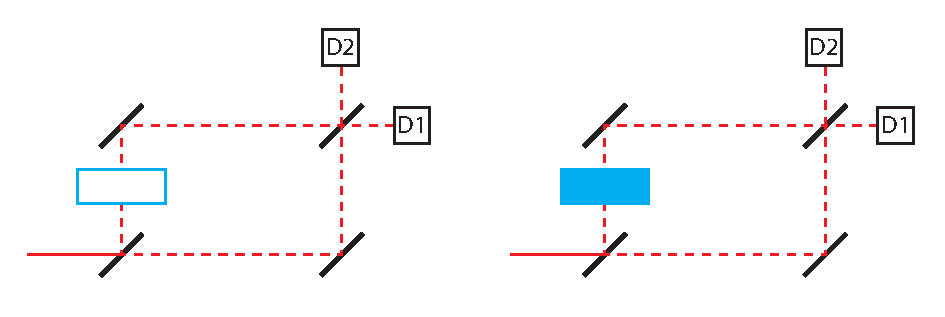
\includegraphics[width=0.75\textwidth]{figures/1.pdf}
    \caption{Иллюстрация к бомбовому парадоксу}
    %\label{fig:}
\end{figure}

Без внешнего влияния срабатывает D1, соответсвенно если мы поставили бомбу, и фотон прилетел в D2, то мы гарантируем, что у нас правильная бомба, при этом фотон через неё не пролетал. 


\textbf{Эффект Зенона}. Настроим вращатель так, чтобы за $N$ пролетов случился поворот на $\pi/2$, тогда вероятность
\begin{equation*}
	P_1 = \left(
		\cos^2 \frac{\pi}{2N}
	\right)^N = \left(1 - \frac{\pi^2}{4 N^2}\right)^N = e^{-\pi/N}.
\end{equation*}
На картинке представлена схема эксперимента. 
\begin{figure}[h]
    \centering
    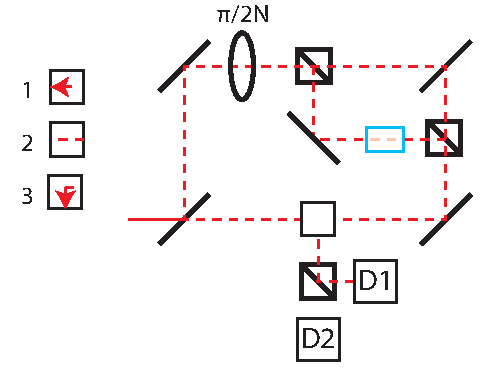
\includegraphics[width=0.3\textwidth]{figures/2.pdf}
    \caption{Эффект Зенона}
    %\label{fig:}
\end{figure}
Таким образом вероятность поглотиться объектом нулевая, однако гарантировано мы при $N \to \infty$ определяем наличие на пути объекта. 